% Options for packages loaded elsewhere
\PassOptionsToPackage{unicode}{hyperref}
\PassOptionsToPackage{hyphens}{url}
\PassOptionsToPackage{dvipsnames,svgnames,x11names}{xcolor}
%
\documentclass[
  12pt,
  letterpaper,
]{article}

\usepackage{amsmath,amssymb}
\usepackage{iftex}
\ifPDFTeX
  \usepackage[T1]{fontenc}
  \usepackage[utf8]{inputenc}
  \usepackage{textcomp} % provide euro and other symbols
\else % if luatex or xetex
  \usepackage{unicode-math}
  \defaultfontfeatures{Scale=MatchLowercase}
  \defaultfontfeatures[\rmfamily]{Ligatures=TeX,Scale=1}
\fi
\usepackage{lmodern}
\ifPDFTeX\else  
    % xetex/luatex font selection
\fi
% Use upquote if available, for straight quotes in verbatim environments
\IfFileExists{upquote.sty}{\usepackage{upquote}}{}
\IfFileExists{microtype.sty}{% use microtype if available
  \usepackage[]{microtype}
  \UseMicrotypeSet[protrusion]{basicmath} % disable protrusion for tt fonts
}{}
\makeatletter
\@ifundefined{KOMAClassName}{% if non-KOMA class
  \IfFileExists{parskip.sty}{%
    \usepackage{parskip}
  }{% else
    \setlength{\parindent}{0pt}
    \setlength{\parskip}{6pt plus 2pt minus 1pt}}
}{% if KOMA class
  \KOMAoptions{parskip=half}}
\makeatother
\usepackage{xcolor}
\usepackage[margin=1in]{geometry}
\setlength{\emergencystretch}{3em} % prevent overfull lines
\setcounter{secnumdepth}{-\maxdimen} % remove section numbering


\providecommand{\tightlist}{%
  \setlength{\itemsep}{0pt}\setlength{\parskip}{0pt}}\usepackage{longtable,booktabs,array}
\usepackage{calc} % for calculating minipage widths
% Correct order of tables after \paragraph or \subparagraph
\usepackage{etoolbox}
\makeatletter
\patchcmd\longtable{\par}{\if@noskipsec\mbox{}\fi\par}{}{}
\makeatother
% Allow footnotes in longtable head/foot
\IfFileExists{footnotehyper.sty}{\usepackage{footnotehyper}}{\usepackage{footnote}}
\makesavenoteenv{longtable}
\usepackage{graphicx}
\makeatletter
\def\maxwidth{\ifdim\Gin@nat@width>\linewidth\linewidth\else\Gin@nat@width\fi}
\def\maxheight{\ifdim\Gin@nat@height>\textheight\textheight\else\Gin@nat@height\fi}
\makeatother
% Scale images if necessary, so that they will not overflow the page
% margins by default, and it is still possible to overwrite the defaults
% using explicit options in \includegraphics[width, height, ...]{}
\setkeys{Gin}{width=\maxwidth,height=\maxheight,keepaspectratio}
% Set default figure placement to htbp
\makeatletter
\def\fps@figure{htbp}
\makeatother

% -----------------------
% CUSTOM PREAMBLE STUFF
% -----------------------

% -----------------
% Title block stuff
% -----------------

% Abstract
\usepackage[runin]{abstract}
\renewcommand{\abstractnamefont}{\sffamily\small\bfseries}
\renewcommand{\abstracttextfont}{\sffamily\small}
\setlength{\absleftindent}{5pt}
\setlength{\absrightindent}{\absleftindent}

% Title
\usepackage{titling}
\pretitle{\par\begin{flushleft}\LARGE\sffamily\bfseries}
\posttitle{\par\end{flushleft}\vskip 10pt}

% Keywords
\newenvironment{keywords}
{\small\sffamily{\sffamily\small\bfseries{Keywords.}}}

% Authors
\usepackage{orcidlink}  % Create automatic ORCID icons/links
%\renewcommand{\and}{\end{tabular} \hskip 3em \begin{tabular}[t]{@{\hspace{0em}}l@{}}}
\preauthor{\begin{flushleft}
           \lineskip 1.5em}
\postauthor{\end{flushleft}}

% ------------------
% Section headings
% ------------------
\usepackage{titlesec}
\titleformat*{\section}{\Large\sffamily\bfseries\raggedright}
\titleformat*{\subsection}{\large\sffamily\bfseries\raggedright}
\titleformat*{\subsubsection}{\normalsize\sffamily\bfseries\raggedright}
\titleformat*{\paragraph}{\small\sffamily\bfseries\raggedright}

%\titlespacing{<command>}{<left>}{<before-sep>}{<after-sep>}
% Starred version removes indentation in following paragraph
\titlespacing*{\section}{0em}{2em}{0.1em}
\titlespacing*{\subsection}{0em}{1.25em}{0.1em}
\titlespacing*{\subsubsection}{0em}{0.75em}{0em}

% ------------------
% Headers/Footers
% ------------------
\usepackage{fancyhdr}
\pagestyle{fancy}
\fancyhf{}
\fancyhead[L,C,R]{}
\fancyfoot[L,C]{}
\fancyfoot[R]{\thepage}
\renewcommand{\headrulewidth}{1pt}
\fancypagestyle{plain}{%
    \renewcommand{\headrulewidth}{0pt}%
    \fancyhf{}%
    \fancyfoot[R]{\thepage}%
}
\renewcommand\footnoterule{\rule{\linewidth}{0.1pt}\vspace{5pt}}

% ------------------
% Captions
% ------------------
\usepackage[labelfont=bf,labelsep=period]{caption}
\captionsetup[figure]{font=footnotesize,justification=raggedright,singlelinecheck=false,format=hang}


% ---------------------------
% END CUSTOM PREAMBLE STUFF
% ---------------------------
\usepackage{dcolumn}
\makeatletter
\@ifpackageloaded{caption}{}{\usepackage{caption}}
\AtBeginDocument{%
\ifdefined\contentsname
  \renewcommand*\contentsname{Table of contents}
\else
  \newcommand\contentsname{Table of contents}
\fi
\ifdefined\listfigurename
  \renewcommand*\listfigurename{List of Figures}
\else
  \newcommand\listfigurename{List of Figures}
\fi
\ifdefined\listtablename
  \renewcommand*\listtablename{List of Tables}
\else
  \newcommand\listtablename{List of Tables}
\fi
\ifdefined\figurename
  \renewcommand*\figurename{Figure}
\else
  \newcommand\figurename{Figure}
\fi
\ifdefined\tablename
  \renewcommand*\tablename{Table}
\else
  \newcommand\tablename{Table}
\fi
}
\@ifpackageloaded{float}{}{\usepackage{float}}
\floatstyle{ruled}
\@ifundefined{c@chapter}{\newfloat{codelisting}{h}{lop}}{\newfloat{codelisting}{h}{lop}[chapter]}
\floatname{codelisting}{Listing}
\newcommand*\listoflistings{\listof{codelisting}{List of Listings}}
\makeatother
\makeatletter
\makeatother
\makeatletter
\@ifpackageloaded{caption}{}{\usepackage{caption}}
\@ifpackageloaded{subcaption}{}{\usepackage{subcaption}}
\makeatother
\ifLuaTeX
  \usepackage{selnolig}  % disable illegal ligatures
\fi
\usepackage{bookmark}

\IfFileExists{xurl.sty}{\usepackage{xurl}}{} % add URL line breaks if available
\urlstyle{same} % disable monospaced font for URLs
\hypersetup{
  pdftitle={Navigating Ancestry and Racial Classification Amongst Multiracial Indigenous American},
  pdfauthor={Matthew Guerra},
  pdfkeywords={Indigenous identity, multiracial
studies, ancestry, racial decision-making, racial
classification, settler-colonialism, QuantCrit, American Community
Survey},
  colorlinks=true,
  linkcolor={blue},
  filecolor={Maroon},
  citecolor={Blue},
  urlcolor={red},
  pdfcreator={LaTeX via pandoc}}


\title{Navigating Ancestry and Racial Classification Amongst Multiracial
Indigenous American\thanks{Thanks to everyone for checking this out.}}
% subtitles do not seem to work with article class?
%%\subtitle{}

\author{
{\bfseries \normalsize Matthew Guerra~\orcidlink{0009-0003-2658-442X}}%
\thanks{Corresponding author.} \\%
 \small University of Oregon, Sociology \\%
{\footnotesize \url{mguerra2@uoregon.edu}} \\\vspace{10pt}
}

\predate{}
\postdate{}
\date{}
\begin{document}

% for some reason this does not work in header
\renewcommand{\abstractname}{Abstract.}

% add the short title to the fancy header
\fancyhead[R]{Navigating Ancestry and Racial Classification}

\maketitle
%\noindent \rule{\linewidth}{.5pt}
\begin{abstract}
Current research on race and multiracial individuals recognizes that
Indigenous racial identity is fluid and often contested. Using a
settler-colonial theoretical framework and the recommendations of
QuantCrit literature, this research project expands understanding of
multi-racial Indigenous identity and demonstrates how ancestry
influences racial ``decision-making'' for Indigenous Americans. By
leveraging data from the American Community Survey (ACS) from 2010 to
2020, the relationship between an individuals reported ancestry and
their self-identified racial classification is investigated by
estimating multinomial logistic regression models. The results indicate
the relationship between various predictorss, and a persons likelihood
to identify as Indigenous alone, multi-racial, or to distance themself
from their Indigenous ancestry and identity in favor of their other
racial identity. When these findings are evaluated within the context of
settler-colonialism, many previously confounding findings can be linked
to the social reality that respondents navigate as Indigenous Americans.
\end{abstract}
\begin{keywords}
\def\sep{;\ }
Indigenous identity\sep multiracial studies\sep ancestry\sep racial
decision-making\sep racial
classification\sep settler-colonialism\sep QuantCrit\sep 
American Community Survey
\end{keywords}
%\noindent \rule{\linewidth}{.5pt}

\subsection{Introduction}\label{introduction}

Who is Indigenous and who is not? Where do multiracial Indigenous
Americans fit in that equation? One group of scholars has asked similar
questions in an attempt to better understand Indigenous identity by
determining which factors are associated with strong Indigenous
identity, how this identity is contested and understood at an
interpersonal and community level, and how the Indigenous population has
grown over time (Liebler, 2010; Lucero, 2014; McKay, 2021). Indigenous
identity becomes even more complicated when considering multiracial
Indigenous Americans, which has led to additional research in this area,
although limited. Articles on Indigenous identity generally cover the
racial decision-making process for multiracial Indigenous people in the
United States, since many Indigenous people have mixed racial
ancestries. This social reality requires Indigenous American respondents
to make conscious decisions when listing their race. In the case of
multiracial Indigenous people their known racial ancestry either
conflicts with or affirms their answer, and they must reconcile with
that decision. Understanding this decision-making process is crucial for
gaining insights into contemporary shifts in racial boundary formation
and the individual considerations that shape racial identification for
Indigenous Americans.

Dwanna L. McKay, Kirsten Vinyeta, and Kari M. Norgaard published an
article titled ``Theorizing Race and Settler Colonialism within U.S.
Sociology'' which calls for a critical approach to how race is studied
within Sociology, particularly how the focus on assimilation fails to
confront its violent and often deadly nature for Indigenous Americans
under settler colonialism (2020). Their article established that as
researchers and academics, we are complicit in the erasure of Indigenous
people, and the continued reification of harmful narratives can only be
stopped by engaging with settler colonialism theory when conducting our
research.

These considerations led to the theoretical engagement explored later in
this paper to prepare for a critical and nuanced approach to
quantitative research that has often been critiqued for its inability to
speak to individual experiences. For those who study race, there have
been criticisms of using race as a static category that does not reflect
the social reality of race as a social construct, which parallels the
arguments mentioned above about settler colonialism within the sociology
of race and ethnicity. This dynamic nature of race means that it can and
does change, and is influenced by various social factors and processes
at both the micro and macro level which is why a critical approach to
the interpretation and contextualization of results from quantitative
research is imperative to furthering understanding without sacrificing
reflexivity (Zuberi \& Bonilla-Silva, 2008). Ultimately, since the
structures of racialization and settler-colonialism inform each other,
an analysis of racial decision-making would be incomplete without
considering how Indigenous racial formation came to be in the US.

\subsection{Theoretical Framework}\label{theoretical-framework}

In 2018 the Journal of Race Ethnicity and Education published a special
issue titled ``QuantCrit: Rectifying Quantitative Methods Through
Critical Race Theory'', where various scholars critically engaged with
quantitative research and methods, using CRT to determine whether
quantitative research is capable of being used to further a critical
race agenda in education research and beyond (Garcia et al., 2018). This
approach is not new, however, and has already been established in Du
Bosian sociology, most notably in Du Bois's The Philadelphia Negro and
The Souls of Black Folk. The Philadelphia Negro has been described as a
great example of an alternate approach to quantitative research that can
be liberating and work to counter oppressive racial narratives while
presenting statistical analysis alongside theoretical arguments (Conwell
\& Loughran, 2023). Du Bois's approach came from necessity due to the
popularity of theories like Social Darwinism which placed Black people
at the bottom of the hierarchy, a reality that required the questioning
of assumptions and working against the grain of how quantitative
research was and often continues to be done. In The Souls of Black Folk
Du Bois uses his lived experiences to theorize and explain what it was
to be Black in American society. Emphasizing historical context and
providing an explanation for the differences in perception between Black
Americans and everyone else, most notably through double consciousness,
the veil and the barriers of the color line. In this article, this
approach will be replicated as best as possible, and part of that
requires delving into settler colonial theory and current research
related to Indigenous identity in the U.S. to create a historical and
theoretical context that this paper will rely on to relate and explain
its findings.

In his article ``Settler Colonialism and the Elimination of the
Native,'' Patrick Wolfe describes what he coined the `logic of
elimination' (2006). This logic explains the operation of colonizers
arriving and settling on lands already inhabited by another group,
specifically that settler colonialism requires the implementation of
violence to achieve the goals of a settler society and replace
Indigenous structures with those of the settler society. The replacement
of Indigenous structures ultimately includes the removal and
dispossession of Indigenous people themself, which was justified through
the racialization of Indigenous people which continues today, speaking
to Wolfe's assertion that settler colonialism is a ``structure rather
than an event'' (Gonzales \& Kertész, 2023; Wolfe, 2006, p.~390). Since
the structures of racialization and settler-colonialism inform each
other, an analysis of racial decision-making would be incomplete without
considering how Indigenous racial formation came to be in the US.

For Indigenous Americans, membership within a tribe is often a key part
of this process to distinguish between those who are Indigenous and
those who are not. This concept is demonstrated in research done to
identify what barriers to tribal enrollment exist for individuals who
have been separated from their family and community via adoption and the
foster system (Landers et al., 2021). Tribal enrollment was identified
as key for individuals to establish and prove their own identity and
seek collective identity within the tribe. Essentially, tribal
enrollment exists as a ``process of mutual verification between the
individual and the tribe'' (Landers et al., 2021, p.~1374).~
Additionally, the forceful removal of Indigenous children from their
families between the 1800s and 1970s by the United States federal
government---via relocation, boarding schools, child welfare removal,
adoption era practices, and so on, has created a group of Indigenous
Americans, and their descendants, who have been removed from their
family and culture thus further causing turmoil in how they
conceptualize their identity. The Federal Acknowledgement Project of
1978, furthered this process since it created an administrative process
that required any group wishing to be acknowledged by the federal
government as a legitimate group to meet certain criteria established by
the federal government, further establishing Indigenous American
identity as an administrative process rather than of racial, ethnic, or
cultural identity (Gonzales et al., 2007). The process explained above
is one of the many ways the `elimination of the native' has been
accomplished, although elimination does not mean only the physical
elimination of Indigenous people. For example, in their article
``Settler Colonialism as eco-social structure and the production of
colonial ecological violence,'' Bacon emphasized that settler-colonial
elimination projects are not just limited to traditional perceptions of
genocide but include assimilation (2019). The boarding schools
Indigenous children were forced to attend not only utilized physical
harm and violence but perpetuated colonial ecological violence by
disrupting the passing on of traditional ecological knowledge from elder
to child in favor of knowledge deemed superior by settlers (2019).

Blood quantum exists as a common requirement for tribal membership. The
blood quantum minimum functions as a benchmark of authenticity for who
is recognized as Indigenous by the tribal government and continues to
endure as a key feature of Indigenous identity, and ultimately is an
important part of determining who can access the few resources offered
by the U.S. government such as healthcare and social services through
the Indian Health Service (IHS) and the Bureau of Indian Affairs (BIA)
(McKay, 2021; Rodriguez-Lonebear, 2021). This system of blood quantum
was established as criteria for federal recognition in response to laws
like Virginia's Racial Integrity Act of 1924 and the Indian
Reorganization Act (IRA) of 1934 which helped establish racial divisions
and criteria on how to quantify Indigenous identity, respectively
(Gonzales et al., 2007). The various laws related to blood quantum
establish that determining Indigenous identity functions as an
administrative process rather than a cultural process of a distinct
racial and ethnic group, allowing a governing body to determine who can
identify as Indigenous, the goal is to create an ever-shrinking
population (Lambert, 2019). This concept demonstrated what McKay calls
the American Indian Legal Identity (AILI). This idea is a proxy for an
Indigenous identity borne of legal and federal policy, devoid of
Indigeneity's cultural and community-based components (2013).~

Keeping the history of racial formation for Indigenous Americans in mind
is important to be aware of when going into the results of this
analysis, especially when considering how settler colonial theory can
-both inform and support potential findings. Furthermore, the
interpretation of results through the lens of CRT, QuantCrit, or
settler-colonialism may not be able to account for every finding.
However, engaging with the social reality multiracial Indigenous
Americans navigate only serves to expand and explain current
understandings regarding Indigenous identity, particularly multiracial
Indigenous identity

\subsection{Methods and Data}\label{methods-and-data}

\subsubsection{\texorpdfstring{\emph{Sample Selection and
Data}}{Sample Selection and Data}}\label{sample-selection-and-data}

The data used for this project was compiled from the American Community
Survey (ACS) data for 2010 - 2020. I seek to analyze the race reporting
of individuals who indicate Indigenous ancestry in addition to another
distinct ancestry group. On the ACS, respondents are asked about their
ancestry via the question ``What is this person's ancestry or ethnic
origin,'' and have two lines to list their responses which are manually
typed and inputted as their responses. Respondents are also asked about
their race and can mark one or more racial categories

Before getting into the specifics of sample selection, there is a needed
conversation about terminology. For this study, the term Indigenous is
used in place of the American Indian and Alaskan Native (AIAN) category
for simplicity's sake as it functions as a collective term since this
project does not focus on a specific Nation, reservation, group, and so
on. It should be noted that this is not done to imply Indigenous people
are a monolith rather is a necessity when conducting a project that
seeks to find patterns of racial identification that span across
individual groups as evidence of the unique role of settler colonialism
in the racialization of Indigenous Peoples in the U.S.

Part of the data organization of this project required the
identification of a multiracial population, specifically an Indigenous
multiracial population. First, any respondents that had an artificially
allocated race response were removed, the goal was to make sure the race
response was indicative of the respondents' true racial response. Then
the Goldstein and Morning method was adopted, which relies on looking at
adults' self-reported ancestry. This approach is beneficial since it
does not rely on the race question to identify a multiracial Indigenous
population, identifies a multiracial population that is aware of their
ancestral descent and allows for a detailed response due to the free
response nature of the question. Due to the free response style of the
ancestry question, about 500 unique responses exist which require
collapsing into specific racial ancestries. The U.S. Census follows the
1997 Office of Management and Budget (OMB) standards on race and
ethnicity and lists the following groups: White, Black or African
American, Asian, American Indian or Alaskan Native, and Native Hawaiian
or Pacific Islander. It also includes the Hispanic or Latino ethnic
category. For example, the Black ancestry group was created by combining
all those whose ancestry fell under the groups of African-American,
non-Latin Caribbean, and Sub-Saharan African. The Asian category
included those whose ancestry fell under East, South East Asian, and
South Asian. The White category included those with European, North
African, and Middle Eastern ancestry. Respondents who listed their race
as Latino or Pacific Islander were dropped from the potential
multiracial Indigenous population. The reason for dropping Latino is
that it functions as an ethnic category on the Census/ACS and
respondents of Latino or Hispanic origin can be any race, so Latino does
not indicate a specific racial ancestry that is easily interpretable as
distinct from Indigenous. The issue with the Pacific Islander category
is that since they are Indigenous to their respective nations this could
create the issue of a double Indigenous ancestry group depending on how
respondents perceive their ancestry and to avoid this potential
discrepancy they were also excluded from the sample.

After the final case selection was concluded the sample size was 490,172
respondents. Once this population was identified their ancestry was
compared to their racial response. When reviewing respondents' racial
ancestry and their race response, four distinct identification patterns
were identified) Indigenous alone, which contained respondents that
listed their race solely as Indigenous regardless of their multiracial
ancestry 2) Consistent, which included respondents that acknowledged
their racial ancestry in full by selecting a racial response that
reflected a multiracial identity 3) Other Race Alone, where respondents'
race response did not reflect their Indigenous ancestry and selected
their identity solely as the other race 4) Inconsistent, where
respondents race response did not reflect their racial ancestry in any
capacity. The inconsistent group was dropped from further analysis,
bringing the sample to 478,680 respondents.

\subsubsection{\texorpdfstring{\emph{Analysis}}{Analysis}}\label{analysis}

I use several multinomial logistic regression models to estimate the
relationship between racial ancestry, race response, and the predictor
variables. The dependent variable has three categories of race response:
Indigenous Alone, Consistent (multiracial), and Other Race Alone. The
key independent variable is racial ancestry. The predictor variables are
metropolitan status (unknown status, non-metropolitan area, metropolitan
area), homeland area (binary), educational attainment (less than HS
diploma, HS diploma, some college, 4-year degree or more), gender
(binary), Hispanic origin (binary), and age (continuous, 18+).

\begin{figure}[!t]

\centering{

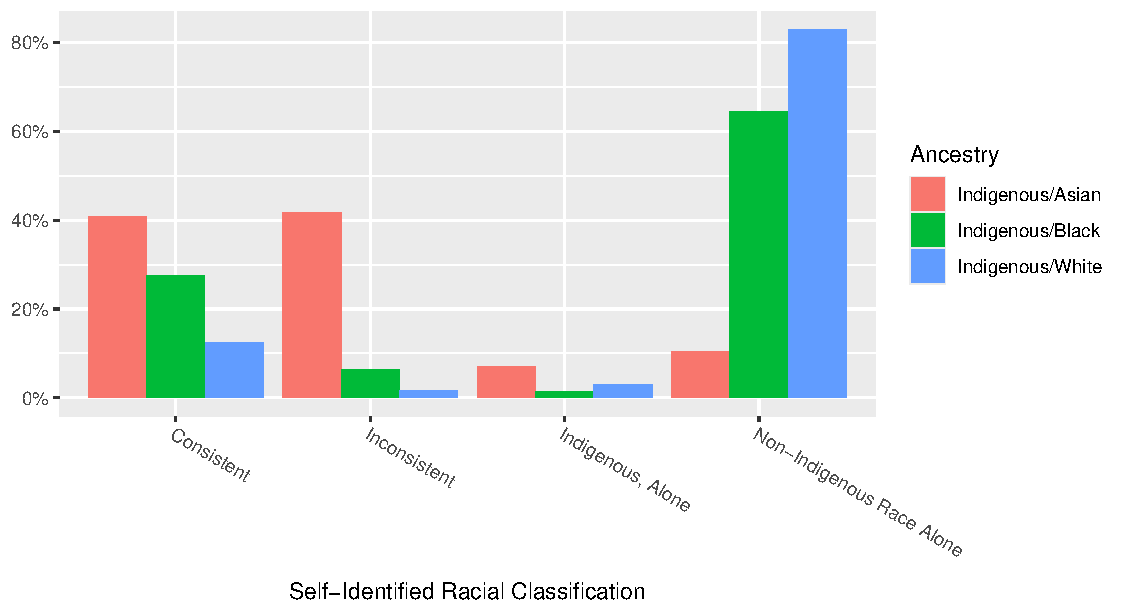
\includegraphics{main_manuscript_files/figure-pdf/fig-race-ancestry-1.pdf}

}

\caption{\label{fig-race-ancestry}Comparing listed ancestry and race
classification}

\end{figure}%

\subsection{Results}\label{results}

\subsubsection{\texorpdfstring{\emph{Multinomial Logistic Regression
Models}}{Multinomial Logistic Regression Models}}\label{multinomial-logistic-regression-models}

My research question focuses on understanding the relationship between
race response and racial ancestry. I use the focal predictor variables
to answer this question by identifying the relationship between the
dependent and independent variables and the predictor variables. Each
table presents coefficients, standard errors, and significance levels
for the multinomial logistic regression models predicting race response
with the predictor variables. The reference group separates these
tables: White and Indigenous, Black and Indigenous, Asian and
Indigenous. The model results compare the predicted race response of
Indigenous Alone and Consistent to Other Race Alone with a separate
table for each ancestry group. The base models of each table look at
racial responses in relation to metropolitan status, the subsequent
model adds Homeland status and the final model educational attainment,
gender, Hispanic origin, and age. This setup creates three sets of
tables with three models each for a total of 9 models total.

\subsubsection{\texorpdfstring{\emph{Metropolitan
Status}}{Metropolitan Status}}\label{metropolitan-status}

Metropolitan status refers to whether respondents live in a metropolitan
area or not. Living in a metropolitan area demonstrated a unique
relationship between each group. For example, it was found that for
respondents with White and Indigenous ancestry, the log odds of
identifying as Indigenous Alone versus White while living in a
metropolitan area were (-0.197). However, once Homeland status was
accounted for it was found that the log odds of identifying as
Indigenous Alone versus White in a metropolitan area is (0.187),
indicating that living in a metropolitan area that is also a Homeland
area is associated with an increased likelihood of an Indigenous
identity. The log odds of respondents identifying as multiracial versus
White when living in a metropolitan area were (0.158). Once Homeland
status is accounted for, living in a metropolitan area increases log
odds of identifying as multiracial versus White (0.348).

For respondents with Black and Indigenous ancestry, living in a
metropolitan area has a negative association with identifying as
Indigenous versus Black (0.708), however, there is a positive albeit
non-significant relationship between metropolitan status and multiracial
identity. Once Homeland status is accounted for this relationship
flipped. Living in a metropolitan area has a non-significant but
negatively associated relationship with identifying as Indigenous versus
Black (-0.206). A significant but positive relationship exists between
living in a metropolitan area and identifying as multiracial versus
Black (0.265).

For respondents with Asian and Indigenous ancestry, living in a
metropolitan area was negatively associated with identifying as
Indigenous versus Asian (-1.769) as well as identifying as multiracial
versus Asian (-0.550). Once Homeland status was accounted for there
continued to be a negative association between identifying as Indigenous
versus Asian (-0.787) and multiracial versus Asian however the
relationship was not significant (-0.103).

Accounting for education, gender, Hispanic origin, and age led to
minimal changes across all three ancestry groups.

\subsubsection{\texorpdfstring{\emph{Homeland
Status}}{Homeland Status}}\label{homeland-status}

LLiving in a location with Homeland status means that a respondent's
household is in an area that includes an area that has been designated
as an American Indian, Alaska Native, or Native Hawaiian (AIANNH) area
(Bureau, n.d.). For respondents with White and Indigenous ancestry,
living on a Homeland was positively associated with identifying as
Indigenous (1.452) and multiracial (0.799) versus identifying as White.
For respondents with Black and Indigenous ancestry living on a Homeland
is positively associated with an Indigenous identity versus Black
(1.177) and the same holds for a multiracial identity versus Black
although not to the same degree (0.509). The Homeland status effect was
strongest for respondents with Asian and Indigenous ancestry, as living
in a Homeland was associated with an increased likelihood to identify as
Indigenous versus Asian(1.900), the same holds for identifying as
multiracial versus Asian (0.843).~

Accounting for education, gender, Hispanic origin, and age led to
minimal changes across all three ancestry groups

\subsubsection{\texorpdfstring{\emph{Educational
Attainment}}{Educational Attainment}}\label{educational-attainment}

Educational attainment consistently has a significant relationship with
race response across ancestry groups, however, three unique patterns
become apparent once a college degree is obtained. For those with White
and Indigenous ancestry obtaining a college degree pushes respondents
away from Whiteness as it is associated with an increase in the log odds
of identifying as Indigenous alone versus White at (0.372) and
Multiracial versus White at (0.328) log odds. For those with Black and
Indigenous ancestry obtaining a college degree pushes respondents away
from Indigenous Alone and towards a Multiracial identity at (-0.355) and
(0.144) log odds respectively. For those with Asian and Indigenous
ancestry obtaining a college degree signaled a move away from
identifying as Indigenous Alone and towards identifying as Asian alone
with the log odds of identifying as Indigenous Alone being (-1.099).

\subsubsection{\texorpdfstring{\emph{Gender}}{Gender}}\label{gender}

Gender demonstrated a unique relationship amongst each of the ancestry
groups. For example, for respondents of White and Indigenous ancestry it
was found that men were more likely to identify as Indigenous or
multiracial versus White at similar rates (0.259 v.~ 0.255).~ When a
respondent has Black and Indigenous ancestry, it was found that gender
did not have a significant relationship between identifying as
Indigenous versus Black but it was found that men are more likley to
identify as multiracial versus identifying as Black than women (0.248).
The opposite effect was seen with those that have Asian and Indigenous
ancestry, as men were found to be less likely to identify as multiracail
versus as Asian than women (-0.300).

\subsubsection{\texorpdfstring{\emph{Hispanic
Origin}}{Hispanic Origin}}\label{hispanic-origin}

In the ACS, Hispanic Origin refers to individuals of
Hispanic/Spanish/Latino origin, where origin is defined by the Census
Bureau as ancestry, lineage, heritage, nationality group, or country of
birth (Bureau, n.d.). Additionally, those of Hispanic Origin can be any
race or any combination of races. In the results of this study, Hispanic
origin is associated with a pattern of increased attachment towards an
Indigenous identity and multiraciality for all ancestry groups.
Respondents who listed White and Indigenous ancestry and are of Hispanic
Origin have increased log odds of identifying as Indigenous Alone versus
White ( 2.161), and the log odds of identifying as Multiracial versus
White are also positive but diminished compared to Indigenous alone
(1.503). Black and Indigenous respondents of Hispanic Origin have
increased log odds of identifying as Indigenous Alone versus Black
(1.691) and similar log odds of identifying as Multriacal versus Black
alone (1.405). Respondents of Asian and Indigenous ancestry who are also
of Hispanic origin have positive log odds of identifying as Indigenous
versus Asian (1.092) as well as multiracial versus Asian (0.804).
Ultimately Hispanic origin increases the likelihood of identifying as
Indigenous or multiracial, yet the effect is strongest to weakest for
those with White and Indigenous ancestry, those with Black and
Indigenous ancestry, and Asian and Indigenous ancestry, respectively.

\subsubsection{\texorpdfstring{\emph{Age}}{Age}}\label{age}

Age as a predictor variable demonstrated minimal effects on racial
response, and significant results were only observed for two ancestry
groups. Amongst respondents with White and Indigenous ancestry it was
observed that for every year in age there was a minimal increase in the
likelihood for respondents to identify as Indigenous versus White
(0.002). The effect was similarly minimal for multiracial versus White
(0.001).

\subsection{Discussion}\label{discussion}

The previously discussed results demonstrated patterns that both
reaffirmed previous findings related to Indigenous identity but also
revealed unique deviations. After further reviewing metropolitan status
three distinct patterns were identified concerning racial identity
responses amongst the three mixed racial ancestry groups.

First, for respondents with both White and Indigenous ancestry, there
was a noticeable shift away from a White identity towards embracing an
Indigenous or a multiracial identity.Second, for those with Black and
Indigenous ancestry, living in a metropolitan area was associated with a
different pattern. These respondents tended to move away from an
Indigenous identity and towards identifying as Black, while
multirciality remained an option at a similar rate of association.
Finally, for respondents with Asian and Indigenous ancestry,
metropolitan status correlated with a tendency to move away from
identifying with their Indigenous ancestry and~ towards identifying
exclusively as Asian rather than multiracial or Indigenous alone.

\begin{itemize}
\item
  living in urban spaces is associated with the creation of a unique
  identity that does not exist without tension (Malika et al., 2024).
\item
  Discuss urban migration and relation to settler colonialism
  (Rosenthal, 2012)
\item
  Tensions of multiracial identity and assertion of agency through
  racial decision making (selection one option or another or choosing
  both) (Cardwell et al., 2020)
\end{itemize}

Homeland Status

\begin{itemize}
\item
  Homeland status increased likelihood to identify as Indigenous for all
  groups, in order of effect WI, AI, and BI, also movement towards
  multiracial
\item
  Liebler Liebler Liebler

  \begin{itemize}
  \item
    Homelands and Indigenous Identity
  \item
    History, place, and racial self-representation in 21st century
    America
  \item
    Challenge with the discussion of tribal sovereignty in enrollment
  \end{itemize}
\item
  Native DNA, relate to sovereignty, relations, connection, enrollment
  rather than focusing on determining authenticity due to blood quantum
  standards ie churning race liebler article

  \begin{itemize}
  \item
    The blood line: racialized boundary making (Rodriguez-Lonebear,
    2021)
  \item
    Native American DNA (TallBear, 2013)
  \item
    Maybe this can connect to sovereignty: Tribal Sovereignty and the
    Limits of Race for American Indians (Small-Rodriguez \& Rocha
    Beardall, 2023)
  \end{itemize}
\end{itemize}

Hispanic Origin

\begin{itemize}
\item
  Latinization of indigenous identity (Campbell-Montalvo, 2023)
\item
  The distinction between indigenous and Latino/Hispanic identity
  (Ybarra, 2023)

  \begin{itemize}
  \tightlist
  \item
    Why do some keep it one but not the other?
  \end{itemize}
\item
  How migration studies can reproduce the logic of elimination, work
  against the idea that when Indigenous people travel they are no longer
  indigenous as explanation for hispanic origin and indigeneity
  relationship (Blackwell et al., 2017)
\end{itemize}

Educational Attainment

\begin{itemize}
\item
  College education pushed WI away from a White identity, for BI pushed
  towards multiracial identity and Black identity, for AI college
  education pushed towards Asian identity

  \begin{itemize}
  \tightlist
  \item
    Potential identity tension?
  \end{itemize}
\item
  Escbach found that people with higher level of education found
  Indigenous identity more appealing, especially in metropolitan areas
  (Eschbach et al., 1998)
\item
  ``With the exception of Black Native Americans, all of the Native
  American male groups have lower levels of schooling''; ``With the
  possible exception of Black Native American women, all groups of
  Native American men and women have some sort of disadvantage in terms
  of schooling or earnings'' (Huyser et al., 2010)

  \begin{itemize}
  \tightlist
  \item
    Seems consistent with findings for BI respondents across gender
  \end{itemize}
\item
  AI is where I am most interested and wondering how much identity
  conflict/tension exists

  \begin{itemize}
  \item
    Are respondents choosing race that matches with stereotypes? I feel
    like that is too simple of an answer, perhaps perception of
    perpetual foreigner leads to more attachment to Asian identity?
  \item
    Racial and ethnic stratification in educational achievement and
    attainment (Kao \& Thompson, 2003)
  \item
    ``The second contemporary pattern of multiracial identification we
    discern might be called simply the ``new'' or even ``immigrant''
    regime whereby a multiple-race label is selected. This convention
    seems to dominate among all the groups of partial Asian ancestry''
    (Gullickson \& Morning, 2011), this continues to be true as can be
    seen in Figure 1 (i haven't named them yet lol)
  \end{itemize}
\end{itemize}

Gender

\begin{itemize}
\item
  I need to look more into research between multiraciality and gender,
  indigenous identity and gender, etc
\item
  Not sure how to approach yet
\end{itemize}

Age

\begin{itemize}
\item
  Age did not have major effect, however thinking in cohorts should be
  interesting
\item
  WI group saw increase to both multiracial and Indigenous identity with
  each year in age
\item
  BI only sees negative association with multiraciaity versus
  identifying just as Black

  \begin{itemize}
  \tightlist
  \item
    One drop rule having more salience for older cohort/groups?
  \end{itemize}
\end{itemize}

\subsection{References}\label{references}



\end{document}
